%%% Laboratory	 Notes
%%% Template by Mikhail Klassen, April 2013
%%% Contributions from Sarah Mount, May 2014
\documentclass[a4paper]{tufte-handout}
\usepackage{tikz}

\newcommand{\workingDate}{\textsc{April $|$ 2022}}
\newcommand{\userName}{A.Belcaid}
\newcommand{\institution}{ENSA-Safi}
\newcommand{\E}{\mathbf{E}}

\usepackage{lab_notes}

\usepackage{hyperref}
\hypersetup{
    pdffitwindow=false,            % window fit to page
    pdfstartview={Fit},            % fits width of page to window
    pdftitle={Correction TD 6},     % document title
    pdfauthor={A.Belcaid},         % author name
    pdfsubject={},                 % document topic(s)
    pdfnewwindow=true,             % links in new window
    colorlinks=true,               % coloured links, not boxed
    linkcolor=DarkScarletRed,      % colour of internal links
    citecolor=DarkChameleon,       % colour of links to bibliography
    filecolor=DarkPlum,            % colour of file links
    urlcolor=DarkSkyBlue           % colour of external links
}


\title{Solution TD 6}
\date{2022}

\begin{document}
\maketitle

\renewcommand{\P}{\mathbf{P}}
% \tikzstyle{probM}[draw]

\section{Loi de probabilite}

Pour que $\P_X$ definit une loi de probabilite il faut que:

\begin{eqnarray*}
1& = & \sum_x \P_x(x) \\
1 & = & \P_x(-3) + \P_x(-2) + \P_x(-1) + \P_x(3) + \P_x(2) + \P_x(1)\\
               1 & = & 2\left(\frac{9}{a}\right) + 2\left(\frac{4}{a}\right) +
               2\left(\frac{1}{a}\right)\\
                 & = & \frac{28}{a}
\end{eqnarray*}
Ainsi 
$$
a = 28
$$.
\begin{marginfigure}
\begin{center}
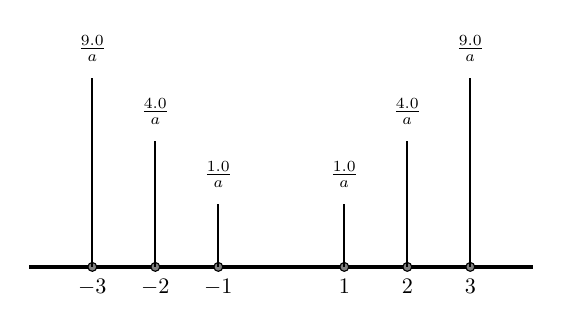
\begin{tikzpicture}[scale=.8, transform shape]
  \path[draw,-,very thick] (-4,0) -- (4,0);
   \foreach \x in {-3, -2, -1, 1, 2, 3}
   { 
     \node[draw, fill=gray, minimum width=4pt, circle, inner sep=0pt,
       label=below:$\x$] at (\x, 0) {};
     \pgfmathsetmacro\ax{abs(\x)}
     \pgfmathsetmacro\xx{pow(\x,2)}
     \path[draw, thick] (\x,0) -- (\x, \ax)node[label=above:{$\frac{\xx}{a}$}]{};
     
   }
\end{tikzpicture}
\end{center}
\caption{Loi de $X$}%
\end{marginfigure}

Soit $Z = X^2$, on cherche la loi de probabilite de $Z$.
  On a:
  \begin{equation*}
    \P_Z(k) = \P_X(x^2 = k)
  \end{equation*}
  Ainsi l'ensembles des valeurs $k$ que peut prendre $Z$ est $\left\{1, 4,
  9\right\}.$

  On obtient alors:

  \begin{equation*}
    P_Z(k) = \begin{cases}
      \frac{2}{28}    & k = 1\\[4pt]
      \frac{4}{28}    & k = 4\\[4pt]
      \frac{18}{28}    & k = 9\\[4pt]
    \end{cases}
  \end{equation*}
\begin{marginfigure}
\begin{center}
\begin{tikzpicture}[scale=0.5]
  \path[draw,-,very thick] (-0,0) -- (10,0);
   \foreach \x/\y in {1/1, 4/4, 9/18}
   { 
     \node[draw, fill=gray, minimum width=4pt, circle, inner sep=0pt,
       label=below:$\x$] at (\x, 0) {};
     \pgfmathsetmacro\ax{abs(\x)}
     \pgfmathsetmacro\xx{2*\x}
     \path[draw, thick] (\x,0) -- (\x, \ax)node[label=above:{$\frac{\xx}{a}$}]{};
     
   }
\end{tikzpicture}
\end{center}
\caption{Loi de $Z$}%
\end{marginfigure}

\section{Loi d'un de truque}
La variables $X$ prend des valeurs dans $\left\{1,2,\ldots,6\right\}$. Par
hypothese, il existe un reel $a$ tel que 

$$
 \P_X(k) = ka
$$

Ce reel doit verifier la relation:

\begin{eqnarray}
  \sum_{x=1}^6 \P_X(x) &=& 1\\ 
  a \times \left(\frac{6\times 7}{2}\right) & = & 1\\
  \frac{21}{a}  & = & 1
\end{eqnarray}
D'ou $ \mathbf{a} = \frac{1}{21}$

On obtient ainsi la loi suivante:

\begin{table}[htpb]
  \centering
  % \caption{ Loi de distribution du de}
  $$
  \begin{array}{ccccccc}
    \toprule
    k & 1 & 2 & 3 & 4 & 5 & 6\\[4pt]
    \midrule
    \P_X(x=k) & \frac{1}{21}& \frac{2}{21} & \frac{3}{21} & \frac{4}{21} &
    \frac{5}{21} & \frac{6}{21}\\[4pt]
    \bottomrule
  \end{array} 
  $$
\end{table}

Calculons maintenant l'\textbf{esperance} de $X$.

\begin{eqnarray*}
  \mathbf{E}[X] &=& \sum_{x=1}^6 x\P_X(x)\\
                &=& \frac{1}{21} \sum_{x=1}^6 x^2\\
                &=& \frac{91}{21}\\
                &=& \frac{13}{3}
\end{eqnarray*}

Soit $Y$ une variable definie par $\frac{1}{X}$. Alors la loi de $Y$ est donne
par:

\begin{table}[htpb]
  \centering
  \caption{Loi de probaiblite de $Y$}
  \label{tab:label}
  $$
  \begin{array}{ccccccc}
    \toprule
    \frac{1}{k} & \frac{1}{1} & \frac{1}{2} & \frac{1}{3} & \frac{1}{4} &
    \frac{1}{5} & \frac{1}{6}\\[4pt]
    \midrule
    \P_Y(=k) & \frac{1}{21}& \frac{2}{21} & \frac{3}{21} & \frac{4}{21} &
    \frac{5}{21} & \frac{6}{21}\\[4pt]
    \bottomrule
  \end{array}
  $$
\end{table}

Si on calcule l'esperance de $Y$, on trouve:
\begin{equation}
  \mathbf{E}(Y) = \frac{2}{7}
\end{equation}

Le but est d'introduire aux etudiantes l'erreur classique que 
$$
\mathbf{E}\left(g\left(X\right)\right)  \neq g(\mathbf{E}\left(X\right))
$$


\section{Deux des a trois faces}

\begin{itemize}
  \item L'espace d'etats des variablesd $(X_1,X_2)$ possedent $9$ resultat
    equiprobables. On peut constuire la loi de la variable $X$ pour chaque
    valeur que peut prendre cette variable aleatoire. on obtient alors:

    $$
    \P_X(x) =\begin{cases}
      \frac{1}{9} & x\in \{-2,2\}\\[4pt]
      \frac{2}{9} & x\in \{-1, 1\}\\[4pt]
      \frac{3}{9} & x = 0\\[4pt]
      0           & \text{sinon}
    \end{cases}
    $$

    Pour l'esperance on as:\footnote{On peut voir aussi que l'esperance est
    nulle car la loi est centree en $0$. Ou parce que $\E[X_1]= \E[X_2]$ ainsi
  on obtient $\E[X_1 - X_2] = \E[X_1] - \E[X_2] = 0$.}

\begin{eqnarray*}
  \E[X] & = & \sum_{x=-2}^2  x\P_X(x)\\[4pt]
        & = & (-2)\cdot \frac{1}{9} + (-1)\cdot \frac{2}{9} + 
(0)\cdot \frac{3}{9} + (1)\cdot \frac{2}{9} + (2)\cdot \frac{1}{9}\\
        & = & 0
\end{eqnarray*}


Pour calculer la \textbf{variance}, on calcule tout d'abord 

\begin{eqnarray*}
  \E[X^2] & = & \sum_x x^2\P_X(x)   \\[4pt]
          & = & (4)\cdot\frac{1}{9} + (1)\cdot\frac{2}{9} + 
(0)\cdot\frac{3}{9} + (1)\cdot\frac{2}{9} + (4)\cdot\frac{1}{9}\\
          & = & \frac{4}{3}
\end{eqnarray*}

\item On pose $Y=X^2$ et on construit la loi de $Y$ en calculant les
  probabilites de toutes les valeurs de $Y$.

  \begin{equation*}
    \P_Y(y) = \begin{cases}
      \frac{2}{9}  & y = 4\\[2pt]
      \frac{4}{9}  & y = 1 \\[2pt]
      \frac{3}{9}  & y = 0 \\[2pt]
      0            & \textbf{sinon}
    \end{cases}
  \end{equation*}

  \begin{marginfigure}
      \centering
      \begin{tikzpicture}
        \draw[thick] (-1,0) -- (5,0)node[label=right:{$Y$}]{};
        \draw[draw,thick] (0,0) -- (0,3)node[label=above:{$\frac{3}{9}$},
          fill=gray,draw,circle]{};

        \draw[draw,thick] (1,0) -- (1,4)node[label=above:{$\frac{4}{9}$},
          fill=gray,draw,circle]{};

        \draw[draw,thick] (4,0) -- (4,2)node[label=above:{$\frac{2}{9}$},
          fill=gray,draw,circle]{};
      \end{tikzpicture}
      \caption{Loi de probabilite de $Y$}
  \end{marginfigure}
  

\end{itemize}
\section{Cles}

\begin{enumerate}
  \item 
Calculer la loi de probabilite de $X$, revient a calculer les nombres
$\mathbf{P}(X=k)$ pour $k = 1, 2,3,4$.

on as 
\begin{eqnarray*}
  \mathbf{P}(X = 1) & = & \frac{1}{4}\\
  \mathbf{P}(X = 2) & = & \frac{3}{4}\cdot\frac{1}{3} = \frac{1}{4}\\
  \mathbf{P}(X = 3) & = & \frac{3}{4}\cdot\frac{2}{3}\cdot\frac{1}{2} = \frac{1}{4}\\
  \mathbf{P}(X = 4) & = &\frac{3}{4}\cdot\frac{2}{3}\cdot\frac{1}{2} = \frac{1}{4} \\
\end{eqnarray*}
Ainsi $X$ une variable uniforme de parametres $\{1, 4\}$.
\item Pour le calcul, de l'esperance, on peut soit 
  \begin{itemize}
    \item Calculer directement:
      $$
      \mathbf{E}(X) = \sum_x P_X(x)x = \frac{1}{4} + \frac{2}{4} + \frac{3}{4} +
      \frac{4}{4} = \frac{5}{2}
      $$
    \item Soit utiliser le resultat demontre qui indique que:

      $$
      \mathbf{E}(X) = \frac{a +b}{2} = \frac{5}{2}
      $$
  \end{itemize}
\item Calculons maintenant la \textbf{variance} de $X$:
      
    \begin{eqnarray*}
      \textbf{Var}(X) &=& \textbf{E}(X^2) - (\mathbf{E}(X))^2\\
                      &=& \frac{1}{4}\left(1 + 4 + 9 + 16\right)- \frac{5}{2}\\
                      &=& \frac{5}{4}
    \end{eqnarray*}
\end{enumerate}

\section{Loi de Pascal}

\begin{enumerate}
  \item Calculer de la loi de $X$.
    On as 
    \begin{eqnarray*} 
      \mathbf{P}(X = k) &=& \mathbf{P}(\text{ k-1 Echecs puis success})\\
                        &=& (1-p)^{k-1}p
    \end{eqnarray*}
    C'est la loi \textbf{geometrique}.
  \item Calculons l'esperance de $X$. On pose tout d'abord $\mathbf{q = 1-p}$.
    \begin{eqnarray*}
      \mathbf{E}(X) &=& \sum_{k=1}^\infty k (1-p)^{k-1}\;p\\
                    &=& p \sum_{k=1}^\infty k\;q^{k-1}\\
                    &=& p \sum_{k=1}^\infty \frac{d}{dq}q^k\\
                    &=& p \frac{d}{dq} \sum_{k=1}^\infty q^k\\
                    &=& p \frac{d}{dq}\left(\frac{q}{1-q}\right)\\
                    &=& p \frac{1}{(1-q)^2}\\
                    &=& \frac{1}{p}
    \end{eqnarray*}
  \item On demontre la propriete de \textbf{sans memoire} de cette loi. Soient
    $k > j $.  On calcul
    \begin{eqnarray*}
      \mathbf{P}(X > k \;|\; X > j) &=& \frac{\mathbf{P}\left( (X>k) \cap (X >
      j)\right)}{\mathbf{P}(X > j)}\\[4pt]
       &=& \frac{\mathbf{P}\left( (X>k)\right)}{\mathbf{P}(X > j)}\\[4pt]
       &=& \frac{(1-p)^k}{(1-p)^j}\\
       &=& (1-p)^{k-j}\\
       &=& \mathbf{P}(X > k -j)
    \end{eqnarray*}
  \item Soit $Y$ la variable aleatoire de l'offre d'achat. On pour chaque entier
    $n$ on as:

    $$
    \mathbf{P}_N(N = n) = \left(\mathbf{P}(Y < K)\right)^{n-1}\underbrace{\mathbf{P}\left(Y>K\right)}_{p}
    $$
    Ainsi $N$ est est une variable aleatoire qui suit une loi
    \textbf{geometrique} de parametre $p$.\\

  Son esperance est donne par $\frac{1}{p}$.
\end{enumerate}

\section{Couple de variables}

\begin{itemize}
  \item A partir de loi jointe de $X$ et $Y$, les elements qui possedent une
    masse sont $(1,1),\; (1,3),\; (2,1),\; (2,3),\; (4,1),\; (4,3)$. Puisque la
    sommes des probabilites doit etre egale a $\mathbf{1}$, on obitent

    \begin{eqnarray*}
      c(1+1)^2 +  c(1+3)^2 + c(2+1)^2 + c(2+3)^2 +  c(4+1)^2 + c(4+3)^2 &=& 1\\
      c\cdot(128) & = & 1
    \end{eqnarray*}
    Ainsi on obtient $c = \frac{1}{128}$.
  \item Les seuls trois instances qui verifient $y < x$ sont $(2,1),\; (4,1),\;
    (4,3)$.
    Ob obtient alors:
    $$
    \P(Y < X) = \P_{XY}(2,1) + \P_{XY}(4,10 + \P_{XY}(4,3) = \frac{83}{128}
    $$
    
  \item On possede un seul etat ou $X = Y$. avec $(x,y) = (1,1)$.
    $$
    \P(X = Y) = \P_{XY}(1,1) = \frac{4}{128}
    $$

  \item La loi de probabilite marginale de $X$ est donnee par $\P_X(x) = \sum_y
    \P_{XY}(x,y).$. 

    Si on applique cette regle pour $x=2$. on obtient

    $$
    \P_X(2) = \P_{XY}(2,1) + \P_{XY}(2,3) = \frac{34}{128}
    $$

    On peut construire toute la loi de $\P_X$:

    $$
    \P_X(x) = \begin{cases}
      \frac{20}{128}   & \text{si } x =1\\
      \frac{34}{128}   & \text{si } x =2\\
      \frac{74}{128}   & \text{si } x =4\\
      0    & \text{sinon } \\

    \end{cases}
    $$
  \item On as :

    $$
    \E[X] = \sum_x x\P_X(x) = 1\cdot \frac{20}{128} + 2\cdot \frac{34}{128} +
4\cdot \frac{74}{128} = 3
    $$
  \item On utilise la definition:

    \begin{eqnarray*}
      \E[XY] & = & \sum_x\sum_y xy\P_{XY}(x,y)  \\
             & = & 1\cdot \frac{4}{128} + 2\cdot \frac{9}{128}
             + 4\cdot \frac{25}{128} 
            + 3\cdot \frac{16}{128}
           + 6\cdot \frac{25}{128}
           + 12\cdot \frac{49}{128}\\[4pt]
             &= & \frac{227}{32}
    \end{eqnarray*}
  \item On utilise la definition directe de la variance:

    $$
    \text{Var}(X) = (1-3)^2 \frac{20}{128} + (2-3)^2 \frac{34}{128} + (4-3)^2
    \frac{74}{128} = \frac{47}{128}
    $$
\end{itemize}

\end{document}


